\documentclass[12pt]{article}

% This first part of the file is called the PREAMBLE. It includes customizations and command definitions. The preamble is everything between \documentclass and \begin{document}.

\usepackage[margin=1in]{geometry}  % set the margins to 1in on all sides
\usepackage{graphicx}              % to include figures
\usepackage{amsmath}               % great math stuff
\usepackage{amsfonts}              % for blackboard bold, etc.
\usepackage{amsthm}                % better theorem environments
\usepackage[english]{babel}
\usepackage{mathtools}
\usepackage{tikz-cd}


% various theorems, numbered by section

\newtheorem{thm}{Theorem}[section]
\newtheorem{lem}[thm]{Lemma}
\newtheorem{prop}[thm]{Proposition}
\newtheorem{cor}[thm]{Corollary}
\newtheorem{conj}[thm]{Conjecture}
\newtheorem{mydef}[thm]{Definition}

\theoremstyle{definition}
\newtheorem{definition}{Definition}[section]

\theoremstyle{remark}
\newtheorem*{remark}{Remark}

\DeclarePairedDelimiter\set\{\}
\newcommand      {\Nm}         {{\mathbb N}}
\newcommand      {\Zm}         {{\mathbb Z}}
\newcommand      {\Qm}         {{\mathbb Q}}
\newcommand      {\Rm}         {{\mathbb R}}
\newcommand      {\Cm}         {{\mathbb C}}
\newcommand      {\vb}        {\mathbf}
\newcommand      {\PP}        {{\mathscr P}}
\newcommand      {\Fm}          {{\mathbb F}}
\newcommand {\lines}[1] {\foreach \n in {1,...,#1}{ \vspace{9mm} \hrule height 
0.2pt  }\vspace{2mm} }


\begin{document}
\bibliographystyle{plain}

%Category Theory: What is a category? What are some examples? How do vector spaces fit into the language of
%category theory? What are some linear algebra concepts that can be viewed as functors in category theory? From
%the viewpoint of category theory how do vector spaces differ from objects such as sets and groups?

\title{Category Theory}

\author{Kevin Guillen \\ 
Department of Mathematics \\
University of California at Santa Cruz \\
Santa Cruz, CA 95064 USA}

\maketitle

\begin{abstract}
    We give an introduction into Category Theory by answering questions such as: What is a category? What is a functor? What can you do with categories? We also focus our examples towards ideas one can find in linear algebra by showing how one may create vector spaces through functors, and relationships between vector spaces through functors. 
\end{abstract}

\section{Introduction}

Category theory was founded around the 1940's by two mathematicians Saunders MacLane and Samuel Eilenberg. It allows mathematicians to study the relationships between different kinds of mathematical objects that typically would show up in very different areas of math. Its prominence came from the slow realization that it is the perfect tool to answer questions in fields such as algebraic topology, homotropy theory, and algebraic geometry. It is very abstract in nature so it seems like it almost describes nothing, which is why it was at times called "abstract nonsense". Today, category theory has grown, and continues to grow, into a very important not only in mathematical areas such as topology, abstract algebra, and representation theory, but even in theoretical computer science and physics. With some historic context out of the way we will begin by defining what is a \textit{Category}.

\section{Categories}
\begin{definition}[Category]
    A \textit{Category} $\mathcal{C}$ consists of the following,
\begin{itemize}
    \item{(1)} a class of objects denoted by \textit{Ob}$(\mathcal{C})$
    \item{(2)} a class of \textit{morphisms} between the objects denoted by Hom$(\textit{Ob}(\mathcal{C}))$
    \begin{itemize}
     \item{}for every object $X,Y$ in \textit{Ob}$(\mathcal{C})$, we have the class Hom$_\mathcal{C}(X,Y) = $ Hom$(X,Y)$ of morphisms. This denotes the subclass of \textit{morphisms} in Hom$(\textit{Ob}(\mathcal{C}))$
    \end{itemize}
    \item{(3)} for any three objects $X,Y,Z$ in \textit{Ob}$(\mathcal{C})$, \[\text{Hom}(Y,Z) \times \text{Hom}(X,Y) \to \text{Hom}(X,Z), \ (f,g) \mapsto f\circ g\] is called a composition and satisfy these axioms,
    \begin{itemize}
        \item{i.} The composition is associative: $f\circ (g\circ h) = (f\circ g) \circ h$ 
        \item{ii.} For every $X$ in \textit{Ob}$(\mathcal{C})$ there is a morphism $1_X$ in Hom$(X,X)$ that is referred to as the unit morphism such that $1_X \circ f = f$ and $g\circ 1_x = g$ for any $f,g$ for which composition makes sense.  
        \item{iii.} If $W,X,Y,Z$ are objects of \textit{Ob}$(\mathcal{C})$ and $(W,X) \neq (Y,Z)$ then Hom$(W,X) \cap \text{Hom}(Y,Z) = \emptyset$
    \end{itemize}
\end{itemize}
\end{definition}

\begin{remark}
    When the term \textit{arrows} or \textit{maps} is said it is talking about morphisms
\end{remark}

This definition is still abstract, so we shall bring up some concepts to help give an idea of what motivated this definition/construction.

Let's move into the realm of abstract algebra. The first exposure one gets to the field is group theory and after we learn about mappings between groups, specifically group homomorphisms. We can also think about the algebraic structures called rings and the ring homomorphisms that come with them. 
We can also think about topological spaces in the field of topology, and how one can construct continuous maps between topological spaces. Lastly when studying vector spaces one can also construct linear maps between these spaces. 

In essence when moving through these different fields of mathematics one sees this pattern of studying some structure and how one can \textit{morph} it to another structure of the same type while preserving important properties.
\vspace{.5cm}

\noindent\textbf{Example 2.1} The following table contains some examples of categories and their morphisms. 

\begin{center}
    \begin{tabular}{ |c|c|c| } 
     \hline
     Category & Objects & Morphisms   \\ 
     \hline \hline
     \textbf{Grp} & groups & group homomorphisms  \\ 
     \hline
     \textbf{Ring} & rings & ring homomorphisms  \\ 
     \hline 
     \textbf{Top} & topological spaces & continuous functions \\
     \hline
     \textbf{Set} &  sets & arbitrary maps \\ 
     \hline
     $\boldsymbol{\textbf{Vect}_k}$ & vector spaces over a field $k$ & linear maps \\
     \hline
    \end{tabular}
\end{center}


There are many other categories one can study, but this should be enough for our focus since we are mostly going to concern ourselves with these categories.

With all this in mind, it makes sense why Category theory is often regarded as a "bird's eye view" of mathematics, since at this level of abstraction, we are not concerning ourselves with the little details pertaining to each specific structure, but rather noticing the patterns between these structures and their respective maps. In the next section we will discuss one of these patterns by first putting away the definition of a category for now. 
\newpage
\subsection{Universal Property} This $\textit{Universal Property}$ is something that we can find in many areas of mathematics. To get into it, let us first consider the set 1. The set 1 represents a set with only one element. Now, \underline{for all sets} $S$, we know there exists a unique map from $S$ to 1. Let us define it as $f$,
\begin{align*}
    f: S &\to 1 \\
    s &\mapsto f(s)
\end{align*}
Where $f(s)$ is simply the only element of 1. In other words we map every element in any set $S$ to the only element in 1. The reason we call this unique is because there is no other way to construct another map from $S$ to 1 other than by sending all elements to the single element. 

This type of property we see with the set 1 can be called \textit{universal} because it explains how it relates with all other things that it lives with. In other words a property like this is \textit{universal} since it shows how the object being described relates to the universe it resides in. 
\vspace{0.5cm}

\noindent\textbf{Example 2.1}
Building on this idea, let us consider the ring of integers, $\Zm$. The rings of integers has the property that \underline{for all} rings $R$, there exists a unique homomorphism from $\Zm$ to $R$. We can see it with the following,
\begin{align*}
    f: \Zm &\to R \\
    f(n) &= \begin{cases}
        \underbrace{1 + 1 + \dots + 1}_n & n > 0 \\
        -f(-n)& n < 0 \\
        0 & n = 0 
    \end{cases}
\end{align*}

This is meant to serve as a quick example so I will omit the proof, but it is clear that this is indeed a ring homomorphism. We have the ring homomorphism now we just want to show that it is indeed unique. Assume there does indeed exist another homomorphism $g$ from $\Zm$ to $R$. We can see through the following though,
\begin{align*}
    g(n) &= g(\underbrace{1 + 1 + \dots + 1}_n) && \text{Homomorphisms preserve addition} \\
    &= \underbrace{g(1) + g(1) + \dots +g(1)}_n \\
    &= \underbrace{1 + 1 + \dots + 1}_n = f(n)
\end{align*}  
In the case where $n = 0$, we know by definition homomorphisms also preserve the additive identity, $g(n) = 0 = f(n)$. The same reasoning follows for negative values since homomorphisms also preserve negative values. 

In essence there is only one object satisfying a \textit{universal property}, since anytime there are two objects satisficing a given universal property, one can always construct an isomorphism between the two. This leads us to the following.
\newpage
\begin{lem}
    Let $S$ be a ring with property that \underline{for all} rings $R$ there exists a unique homomorphism from $S$ to $R$, then $S\cong \Zm$. Where any ring $S$ with the property just described will be called \underline{initial}.
\end{lem}
\begin{proof}
    We know that $S$ is given to be \textit{initial}, then by definition we have a unique homomorphism $f$ from $S$ to $\Zm$. 
    Recall that we also showed $\Zm$ contains this property and is therefore initial, meaning we also have a unique homomorphism $g$ from $\Zm$ to $S$

    What this means though, when taking the composition we get,
    \begin{align*}
        g\circ f: S \to S
    \end{align*}
    which is a homomorphism. It is obvious though that the identity map from any ring onto itself is a homomorphism, but $S$ was defined as initial, and therefore $g\circ f = \text{Id}_S$

    Applying the same reasoning the other way we see that $f \circ g = \text{Id}_\Zm$. This makes $f$ and $g$ inverses of each other, and therefore $S \cong \Zm$
\end{proof}

The goal of this is to show the universal property for what it is; we can further demonstrate it by considering examples relating to our class. 

\vspace{.5cm}
\noindent{\textbf{Example 2.2}}
Let $V,\ U,$ and $W$ be $\Fm-$vector spaces. Consider the bilinear map $f$
\begin{align*}
    f: V\times U \to W
\end{align*}
Omitting some details from class about a vector space $T$, we know there is a universal bilinear out of $V\times U$. Consider the following for vector space $T$,
\[\begin{tikzcd}
    {V\times U} & T \\
    &{W} 
    \arrow["\phi", from=1-1, to=1-2]
    \arrow["h", from=1-1, to=2-2] 
    \arrow["\hat{h}", from=1-2, to=2-2]
\end{tikzcd}\]
Where $W$ is any $\Fm$-vector space. This is simply saying that bilinear maps out of $V\times U$ have a 1-1 correspondence with linear maps out of $T$. We know from class that $T$ is just the vector space of the tensor product of $V$ and $U$. The reason for omitting this fact is because without actually knowing that $T$ and $\phi$ exist one can prove that this universal property determines $T$ and $\phi$ uniquely. The proof follows similar reasoning to that of \textbf{Lemma 2.1}.

\begin{lem}
    Let $V$ and $U$ be $\Fm$-vector spaces, and suppose we have the universal bilinear maps out of $V\times U$ $f:V\times U \to T$ and $f':V\times U \to T'$ then there exists a unique isomorphism $g$ from $T$ to $T'$ such that $g\circ f = f'$
\end{lem}
\begin{proof}
    Using the same reasoning as \textbf{Example 2.2}  but in this case $h$ is $f'$ and instead of mapping to $W$ we are mapping to $T'$ this will give us our linear map $g$ from $T$ to $T'$,
    \[\begin{tikzcd}
        &{T} \\
        {V\times U} & T' \\
        \arrow["f'", from=2-1, to=2-2]  
        \arrow["f", from=2-1, to=1-2]
        \arrow["g", from=1-2, to=2-2 ]
    \end{tikzcd}\]
    where $g\circ f = f'$. Note that if we use the universal property of $f'$ we can also obtain a linear map from $T'$ to $T$,
    \[\begin{tikzcd}
        &{T} \\
        {V\times U} & T' \\ 
        &{T}
        \arrow["f'", from=2-1, to=2-2]  
        \arrow["f", from=2-1, to=1-2]
        \arrow["g", from=1-2, to=2-2 ]        
        \arrow["f",from=2-1, to=3-2]
        \arrow["g'",from=2-2, to=3-2]
    \end{tikzcd}\]
    We see if we compose $g'$ with $g$ we get an endomorphism of $T$, but it also is a linear map satisfying $(g' \circ g)\circ f = f$. Recall that the identity map of $T$ composed with $f$ will also lead to the same result: $Id_T \circ f = f$. Then, by definition of the universal property $f$ this type of mapping has to be unique and we have $g'\circ g = Id_T$, then by similar reasoning we have $g\circ g' = Id_{T'}$ and therefore $g$ is indeed an isomorphism.
\end{proof}
    This is a very important proof we have just done for two reasons. One is that it did not really matter what the details of the map were in that we were mostly depending on the universal property to show these maps exist and how they behave between these objects. The second thing is` what we just proved is that there exists only one pair $(T,f)$ with the universal property of \textbf{Example 2.2}. From class we know this to be the $V\otimes U $, which is just the tensor product of $V$ and $U$!

    \subsection{More on Categories} \label{subsection}

    With some important observations out the way let us jump back to talking about categories and their properties. 
    \begin{definition}[Isomorphism]
        Let $f$ be a map from $A$ to $B$ in a category $\mathcal{C}$. $f$ is an isomorphism if there exists a map $g$ in $\mathcal{C}$ from $B$ to $A$ such that $gf = 1_A$ and $fg = 1_B$

        In essence $g$ plays the role of $f$'s inverse: $g = f^{-1}$
    \end{definition}

    One thing to note about the examples provided in \textbf{Example 2.1} is those categories happen to contain objects that are themselves sets with with structure, but in general objects in categories need not be sets with some structure or sets at all. In essence the point of this note is that one doesn't concern themselves with the elements of an object in a category since in it a requirement for the objects of a category to contain elements. We will explain with further examples 

    \textbf{Example 2.3} The category \textbf{1}. This is a category with only 1 object and only the identity map
    \[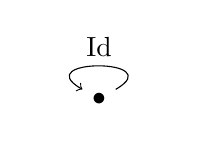
\begin{tikzpicture}
        \node (a) at (0,0) {$\bullet$};
        \draw[->] (a) to[in=150,out=30,looseness=4.8] node[midway,above] {Id} (a);
        \end{tikzpicture}\]
    Now it makes sense to talk about a category with two objects,
    \[\begin{tikzcd}
        \bullet & \bullet
        \arrow["f",from=1-1,to=1-2]
    \end{tikzcd}\]
    We don't actually need to draw the identity map since by definition every object is supposed to have one. In this case we have 2 objects with a single non identity map.

    Note that we mentioned that objects in a category must have the identity map, that means there are categories with no non-identity maps and are typically referred to as \textit{discrete} categories. In this case the objects have no connection to one another; they are lonely. 

    One cool thing that comes from learning about this is that we know in group theory, the first description of groups, and a really common description is that a group is supposed to be the system of all symmetries pertaining to some object. So, if we have some group $G$, say its corresponding category is $\mathcal{C}_G$. We would see that $\mathcal{C}_G$ has 1 object that we can denote as $\bullet$ and the morphisms from $\bullet$ to itself that are given by $G$. 

    Where the morphisms $f$, $g$ from $\bullet$ to $\bullet$ are are composed as $fg:\bullet \to \bullet$

    Now if $\mathcal{C}$ were to be a category with a single object $\bullet$, and every morphism be an isomorphism then Hom$(\bullet,\bullet)$ would form a group $G_\mathcal{C}$. Where the product of group elements is given by the composition of morphisms. 

    The unit element of the group would simply be given by the identity morphism on $\bullet$. Now, one would maybe wonder how the inverse of group elements plays into this and it's simply given by the inverse morphism since every morphism in this category is an isomorphism

    We can think of it with this table,
    \begin{align*}
        \begin{tabular}{ |c|c| }
            \hline
            $\mathcal{C}$ with single object $\bullet$ & group $G_\mathcal{C}$ \\
            \hline
            morphisms in $\mathcal{C}$ & elements of $G_\mathcal{C}$ \\
            \hline
            composition $\circ$ & group operation $\cdot$ \\
            \hline
            $Id_\bullet$ & identity element 1 \\
            \hline
        \end{tabular}
    \end{align*}

    For the following diagram think of every arrow as representing different maps or different elements of the group.
    \[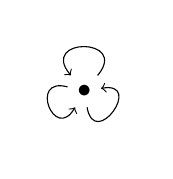
\begin{tikzpicture}
        \node (a) at (0,0) {$\bullet$};
        \draw[->] (a) to[in=130,out=50,looseness=4.8] node[midway,above] {} (a);
        \draw[->] (a) to[in=240,out=165,looseness=4.8] node[midway,left] {} (a);
        \draw[->] (a) to[in = 10, out = 280, looseness = 4.8] (a);
        \end{tikzpicture}\]

    \begin{definition}[Dual]
        Every category has what is called a dual category. For the category $\mathcal{C}$ the dual category of it is $\mathcal{C}$$^{\text{op}}$, which is simply defined by reversing its arrows. 

        Meaning $\textit{Ob}(\mathcal{C}) = \textit{Ob}(\mathcal{C^{\text{op}}})$. Which also means we have for all objects $A$ and $B$ in $\mathcal{C}$ that Hom$_{\mathcal{C}}(A,B)$ = Hom$_{\mathcal{C}^{\text{op}}}(B,A)$. We also have that identities in $\mathcal{C}^{\text{op}}$ are the same as $\mathcal{C}$

        For composition in $\mathcal{C}^{\text{op}}$, it is the same as $\mathcal{C}$, except we have our arguments being reversed. What is meant by this is the following, let $f$ and $g$ be maps in $\mathcal{C}$
        \begin{align*}
            A \stackrel{f}{\to} B \stackrel{g}{\to} C
        \end{align*}
        would be,
        \begin{align*}
            A \stackrel{f}{\leftarrow} B \stackrel{g}{\leftarrow} C 
        \end{align*}
        in $\mathcal{C}^\text{op}$
    \end{definition}

    From this it follows what is called the \textit{principle of duality} which many consider a fundamental principle in category theory. It basically boils down to saying that every categorical definition, theorem, and proof has a dual as well. 

    \begin{definition}[Product Category]
        Let $\mathcal{C}$ and $\mathcal{D}$ be categories. We have the product category $\mathcal{C}\times\mathcal{D}$ as follows,
        \begin{align*}
            ob(\mathcal{C} \times \mathcal{D}) &= ob(\mathcal{C}) \times ob(\mathcal{D}) \\
            \text{Hom}((A,B),(A', B')) &= \text{Hom}(A,A')\times \text{Hom}(B,B')
        \end{align*}
    \end{definition}

    \section{Functors}
    \begin{definition}[Functor]
        A \textit{Functor} $\textbf{F}:\mathcal{C} \to \mathcal{D}$ between categories $\mathcal{C}$ and $\mathcal{D}$ consists of the following,
        \begin{itemize}
            \item{1)} a function,
            \begin{align*}
                \textbf{F}: ob(\mathcal{C}) \to ob(\mathcal{D}) \\
                C \mapsto \textbf{F}(C)
            \end{align*}
            \item{2)} Then for every $A$ and $B$ in $\mathcal{C}$ a function,
            \begin{align*}
                \textbf{F} = \textbf{F}_{A,B}: \text{Hom}(A,B) \to \text{Hom}(\textbf{F}(A), \textbf{F}(B))
            \end{align*}
            which preserves compositions and identity morphisms
        \end{itemize}
        
    \end{definition}

    Taking from common themes in math we know that once we learn about some type of mathematical object we concern ourselves with taking morphisms between that type of mathematical object and others like it. This is in a sense what a functor is doing just at another level of abstraction since now we are concerned with taking maps between different categories. 
    
    

    \noindent{\textbf{Example 3.1}}
    One example of functors or what are called forgetful/stripping functors. Specifically there's a functor $\textbf{U}: \textbf{Grp}\to \textbf{Set}$ which simply takes the underlying set of $G$ and if $f$ were to be a group homomorphism then $\textbf{U}(f)$ is simply $f$ itself. In essence $U$ is just forgetting the group structure of a given group and forgetting group homomorphisms are homomorphisms 

    There is also what is informally called free functors and it's similar to how free is typically used in other branches of math. Relating back to our class if we fix a field $k$ there is a free functor $\textbf{F}: \textbf{Set} \to \textbf{Vect}_k$. It is defined by $\textbf{F}(S)$ being a vector space with its basis $S$. Basically $\textbf{F}(S)$ would be the set of all $k$-linear combinations of elements of $S$. Let $v\in \textbf{F(S)}$, then $v$ can be expressed as,
    \begin{align*}
        v = \sum_{s\in S} \alpha_s s
    \end{align*} where $\alpha_s$ is a scalar. 

    We see $v,w \in \textbf{F}(S) $ can indeed be added through the following,
    \begin{align*}
        v + w = \sum_{s\in S} \alpha_s s + \sum_{s\in S} \beta_s s = \sum_{s\in S} (\alpha_s + \beta_s) s
    \end{align*}
    we also have scalar multiplication for $c\in k$,
    \begin{align*}
        c v = c\sum_{s\in S} \alpha_s s = \sum_{s\in S} (c\alpha_s) s
    \end{align*}
    through this we see $\textbf{F}(S)$ is a vector space

    \begin{definition}[Contravariant functor]
        A contravariant functor from categories $\mathcal{C}$ to $\mathcal{D}$ is a functor $\mathcal{C}^\text{op}\to \mathcal{D}$ 
    \end{definition}

    \noindent{\textbf{Example 3.2}} This is a general example about functors between vector spaces, but in specific cases it relates to an important topic discussed in class and that is the dual space. 

    Let $k$ be a field and $V$ and $W$ be $k$-vector fields. We know Hom$(V,W)$ forms a vector space where the vectors are simply maps. 

    If we fix $W$, any linear map $f: V \to V'$ will induce a linear map $f^{*}: \text{Hom}(V',W) \to \text{Hom}(V,W)$ defined at g in Hom$(V',W)$ by taking $f^{*}(g)$ to simply be the composite of $f$ and $g$.

    Since we have $f$ going from $V$ to $V'$ and $g$ going from $V'$ to $W$

    This actually defines a functor through the following,\[\text{Hom}(\cdot, W): \textbf{Vect}_{k}^\text{op} \to \textbf{Vect}_k\]

    Note what happens when we let $W$ be the $k$-vector space $k$. Then Hom$(V,k)$ would simply be the dual space of $V$. That means there is a contravariant functor \[()^{*} = \text{Hom}(\cdot, k): \textbf{Vect}_k^\text{op} \to \textbf{Vect}_k\] that sends each vector space  to its dual space!

    \section{Conclusion} In all we only managed to get a small taste of what category theory is. We managed to define a category and how one works with a category through its properties and functors. We also managed to provide some examples of how a variety of mathematical objects are view under the lens of category theory, and showcased some linear algebra concepts through the lens of categories and functors. Unfortunately we may have spent a bit too much time talking about the universal property since we couldn't reel it back in perfectly, but it was still a very cool aspect to look at it since it too has a meaning in category theory due to how often it is found in mathematical structures. 

    We also showcased category theory's goal and ability to capture things that are commonly found in different classes of mathematical structures and deducing things using the morphisms found between these structures.  
 
    \textbf{Side Note:} We couldn't make it to discussing any theorems so there's only lemmas, definitions, and examples. 



    
    \begin{thebibliography}{9}
        \bibitem{textbook}
        Brendan Fong, David I. Spivak (2018) \emph{Seven Sketches in Compositionality: An Invitation to Applied Category Theory}, Cambridge University Press.

        \bibitem{textbook}
        Emily Riehl (2016) \emph{Category Theory in Context}, Dover Publications.
        
        \bibitem{textbook}
        Jiri Adamek (2009) \emph{Abstract and Concrete Categories: The Joy of Cats (Dover Books on Mathematics)}, Dover Publications; Illustrated edition.
        
        \bibitem{textbook}
        Tom Leinster (2016) \emph{Basic Category Theory}, arXiv 1612.09375

        \bibitem{textbook}
        Saunders MacLane (1998) \emph{Categories for the Working Mathematician}, Springer; 2nd edition.
        
    
    \end{thebibliography}















\end{document}